\documentclass[preprint]{sigplanconf}

\usepackage[T1]{fontenc}
\usepackage[english]{babel}   
\usepackage[latin1]{inputenc}  
\usepackage{times}
\usepackage{graphicx}
\usepackage{url}
\usepackage{listings}
\usepackage{subfigure}
\usepackage{cite}


\lstloadlanguages{[ANSI]C++,HTML}
\lstdefinelanguage{XML} {
  keywords={xml,version,DOCTYPE,SYSTEM,EPOSConfig,family,member,name,type,
  feature,trait,class,performance,codesize,energy,power,default,pos,pre}}
\lstdefinestyle{prg} {basicstyle=\small\sffamily, lineskip=-0.2ex}
\lstdefinestyle{prgbox} {basicstyle=\small\sffamily lineskip=-0.2ex}
\lstdefinestyle{inlineprg} {basicstyle=\small\sffamily}

\newcommand{\fig}[4][htbp]{
  \begin{figure}[#1] {\centering{\scalebox{#4}{\includegraphics{fig/#2}}}\par}
    \caption{#3\label{fig:#2}}
  \end{figure}
}

\newcommand{\largefig}[4][htb]{
  \begin{figure*}[#1] {\centering{\scalebox{#4}{\includegraphics{fig/#2}}}\par}
    \caption{#3\label{fig:#2}}
  \end{figure*}
}


\newcommand{\prg}[4][htb]{
  \begin{figure}[#1]
%    \vspace{\parskip}
%    \makebox[\textwidth][c]{
      \lstinputlisting[language=#2,style=prg]{prg/#3.prg} %}
%    \vspace{0.4\parskip}
    \caption{#4\label{prg:#3}}
  \end{figure}
}

%\newcommand{\note}[1]{\marginpar{\footnotesize{#1}}}
\newcommand{\note}[1]{}

\begin{document}

\conferenceinfo{EuroSys '07}{Lisbon}
\copyrightyear{2005}
\copyrightdata{[to be supplied]}

\title{Application-Driven Power Management for Embedded Systems}

\authorinfo{Arliones Stevert Hoeller Junior, Lucas Francisco Wanner and Antnio Augusto Frhlich}
           {Laboratory for Software and Hardware Integration\\P.O.Box 476, 88040900\\Florianpolis - Brazil}
           {\{arliones,lucas,guto\}@lisha.ufsc.br}

\maketitle

\begin{abstract}

  Deeply Embedded Systems usually are simple, battery-powered systems
  with resource limitations. In some situations, their batteries
  lifetime becomes a primordial factor for reliability. Because of
  this, it is very important to handle power consumption of such
  devices in a non-restrictive and low-overhead way. This power
  management cannot restrict the wide variety of different low-power
  modes such devices often feature, thus allowing a wider system
  con\-fi\-gu\-ra\-bi\-li\-ty. However, once in such devices
  processing and memory are often scarce, the power management
  strategy cannot compromise large amounts of system resources. In
  this paper we propose a simplified interface for power management
  of software and hardware components. The approach is based on the
  hierarchical organization of such components in a component-based
  operating system and allows power management of system components
  without the need for costly techniques or strategies. A case study
  including real implementations of system and application is
  presented to evaluate the technique and shows energy saves of
  almost 40\% by just allowing applications to express when certain
  components are not being used.

\end{abstract}

%%%%%%%%%%%%%%%%%%%%%%%%%%%%%%%%%%%%%%%%%%%%%%%%%%%%%%%%%%%%%%%%%%%%%%%%%%%%%%%

\section{Introdu��o}
\label{sec:introducao}
% ------------------------------------------------------------------------------
\section{Introduction} \label{intro}
% + Introduction
% 
% The very first letter is a 2 line initial drop letter followed
% by the rest of the first word in caps.
%
% form to use if the first word consists of a single letter:
% \IEEEPARstart{A}{demo} file is ....
%
% form to use if you need the single drop letter followed by
% normal text (unknown if ever used by IEEE):
% \IEEEPARstart{A}{}demo file is ....
%
% Some journals put the first two words in caps:
% \IEEEPARstart{T}{his demo} file is ....
%
% Here we have the typical use of a "T" for an initial drop letter
% and "HIS" in caps to complete the first word.
% \IEEEPARstart{T}{his} demo file is intended.

\IEEEPARstart{E}{nergy} consumption is a determining factor when designing wireless sensor networks.
As a consequence, battery lifetime is a limitation on the development of such systems.
Therefore, the idea of extracting energy from the environment has become attractive.
Looking to the energy consumption problem, the intelligent usage of the stored energy contributes to extend the sensor nodes' longevity.
Consequently, energy schedulers have been developed in order to adequately assess the energy consumption and adapt the system accordingly to the available amount of energy.
The purpose of this work is to adapt a solar energy harvesting circuit to supply energy to low power wireless platforms, i.e., those that operate under $50~mW$.
Simultaneously, we aim at improving the performance of the energy-aware task scheduler in wireless sensor network systems by providing fine-grained battery and environmental monitoring.

Among a number of energy sources that have been studied so far, solar has proved to be one of the most effective~\cite{Roundy:2003}.
The solar energy conversion through photovoltaic (PV) cells is better performed at an optimum operating voltage.
Operating a solar panel on this voltage results in transferring to the system the maximum amount of power available.
In this context, \emph{maximum power point tracker circuits} (MPPT) have been proposed.
The drawback is that MPPT circuitry may introduce losses to a solar harvesting system.
Concerning low-power applications, it may be more energy efficient to have a good matching between the solar panel and the energy storage unit~\cite{Raghunathan:2005}.
This well matched system is than able to work close to the maximum power point with less power loss.

In this work, an evaluation of the proposed harvesting circuit is performed in order to show improvements on an energy-aware task scheduler~\cite{Hoeller:SMC:2011}.
It is shown that the combination of the proposed circuit with the cited scheduler not only extended the longevity of the wireless sensor network, but also improved system quality.

The paper is organized as follows:
Section~\ref{fund} presents the fundamentals of solar energy harvesting and energy-aware task scheduler.
Section~\ref{design} discusses the design of the harvesting circuit under the perspective of low power wireless platforms.
Section~\ref{case} presents the evaluation of the harvesting circuit and a case study showing the improvements on system quality.
Finally, section~\ref{concl} closes the paper.

% ------------------------------------------------------------------------------


\section{O gerente de consumo de energia proposto}
\label{sec:gerente}
\note{Pol�ticas tradicionais analisam dinamicamente o comportamento do
sistema e da aplica��o. APIs (drivers) r�gidas e
incompletas. Padroniza��o num n�vel muito baixo.}

%%% essa afirma��o das APIs/drivers ficou leviana. o foco de critica deveria
%%% ser o 'nivel' da abstracao.

Power management policies in conventional operating system (e.g. Linux,
Windows) dynamically analise the system's behavior in order to determine
when a hardware component should change its operation to a lower or
higher power consumption mode. The software implementation responsible
for those state migrations often rely on hardware-specific interfaces,
which are exported through rigid, and sometimes incomplete APIs
(application programming interfaces) or device drivers. In these
environments, power managing interfaces are standardized in a very low
abstraction level, closer to the actual hardware than the system's
abstractions.


\note{APM e ACPI s�o ``tentativas'' de padroniza��o. Muito usados, definem
interface entre hardware e software. N�o se adaptam a SE.}

%%% A segunda parte ficou muito esquisita, e desconexa. 
%%% Que tem a ver o servidor e o laptop? Porque n�o
%%% d� pra usar o mesmo procedimento do servidor (desligar qd nao usa)
%%% num SE? Acho que perdeu o foco aqui.

Most general purpose computer hardware devices implement either
\textsc{Apm} (\textit{Advanced Power Management}) or \textsc{Acpi}
(\textit{Advanced Configuration Power Interface}) standard interfaces to
allow power management. Although these standards share little in comon,
their objective is the same: to allow devices to be turned on, off or to
be put in a low power consumption mode for a certain period of time.
These techniques work well in environments such as servers that
frequently do not use certain resources or laptop computers, that may
\emph{suspend to disk} or turn off the system when battery charge is
low. These procedures, however, are hardly ever applicable in embedded
systems.

\note{Diversidade da necessidade das aplica��es em termos de consumo
de energia demanda uma granularidade fina de configura��o de modos de
opera��o. PM em computa��o gen�rica foca CPU. SE tem que focar
perif�ricos.}

%%% n�o � o mesmo objetivo nos dois mundos? economizar, permitindo
%%% operar adequadamente?

Most of the resource in power managing interfaces and techniques is
focused on general purpose computer hardware (e.g. personal computers,
servers, laptop and handheld computers), and many research efforts focus
on managing the consumption of the main microprocessor (CPU), as these
devices are responsible for most of the power consumption in these
systems. In embedded systems, however, processors and microcontrollers
are usually very simples, and consume little power. Most of the power
consumed by these systems comes from peripheral devices. Thus, power
managing for these systems must focus on fine grain techniques that
conserve power from peripheral devices, while allowing the system to
operate properly.


\note{An�lise din�mica n�o pode ser comportada. Considerando que a
maioria dos SE rodam apenas uma aplica��o (computa��o dedicada), o
melhor lugar pra determinar a estrat�gia de ger�ncia de energia � na
pr�pria aplica��o}

%%% o texto original estava s� repetindo o que j� tinha sido
%%% dito antes. mudei um pouco, mas acho que ainda n�o t� 100%.

%%% gerente 'ativo' n�o "soa" melhor do que gerente 'dinamico'?

Embedded systems often have to deal with severe resource restrictions,
from restricted hardware capabilities (e.g. memory, processing power) or
functional requirements (e.g. availability, real-time responsiveness).
Thus, most embedded systems cannot afford the cost of dynamic, active
power managers. Previous research \cite{1,2,3,4} indicates that the most
efficient power managing techniques are the ones that take into
consideration the behavior of the target applications for a given
system.  Considering that most embedded system perform specific tasks,
and run a single application~\cite{seilaquem}, we may conclude that the
best place to define a power managing strategy is in the application
itself.

\note{Sumarizar a proposta.}

%%% t� bem explicado, mas n�o fica claro o objetivo. naqueles
%%% itens da introdu��o acho que t� melhor.

In this paper, we present a software infra-structure that allows
application-driven power management for embedded systems. We provide an
uniform, hardware-independent \textsc{API} (\textit{Application
  Programming Interface}) that allows applications to change operating
modes for every component in an embedded operating system. In order to
ensure correct and deterministic behavior, relations and dependencies
regarding power management for every component are formalized through
Petri Networks. This formalization allows high-level analisys of the
power state migration procedures for every component, and stablishes a
message exchange mechanism in which components coordenate to ensure
consistent power state changes in subsystems (e.g. communication,
processing, sensing), or the system as a whole.


\note{Esta se��o descreve a proposta (API, Redes e propaga��o)}

\note{novamente o nome :-)}

This section describes DSPM, an application-driven, Deterministic Static
Power Manager for embeddded systems. We stablish an \emph{Application
  Programming Interface} (API) implemented by every system component,
that allows changes in the component's power state.  \emph{Migration
  Networks} formalize the changes in operating modes of components or
groups of components (subsystems), and controls components instancies,
allowing the system to know every component that is currently in use and
to propagate systemwide changes in operation modes.

\subsection{Power Managing Interface for Software and Hardware Components}


\note{Foi definida uma API que permite acesso das aplica��es aos
  componentes do sistemas, bem como a troca de mensagens entre os
  componentes internos.}

%%% a historia do 'acordar automaticamente' ficou mal-explicada

In our power management strategy, the application programmer is
expected to specify in his source code, whenever ceitain 
components will not be used. Thus, an uniform API to allow power management 
was defined. This interface allows interaction between the application
and the system, between system components and hardware devices,
and directly between application and hardware. In order to
free the application programmer from having to \emph{wakeup}
components whenever they are needed, the power managing mechanism
abstracted by this interface ensures that components return to
their previous operational states whenever they are used.

\largefig{api}{Power Manager API}{.7}

\note{Figura apresentando modos de acesso, dando exemplo em sistema
hipot�tico}

Figure~\ref{fig:api} presents all these interaction modes in a
hipothetical system instance. The application may access a global
component (\texttt{System}) that has knowledge of every other component
in the system (in this case \texttt{IPC}, \texttt{Processing},
\texttt{Sensing} and their respective underlying components), triggering
a system-wide power mode change. Annother way the application may use
this interface is through subsystems (e.g., \textit{Inter-Process
  Communication} (\texttt{IPC}), \texttt{Processing}, \texttt{Sensing}). In this
way, messages are propagated only to the components used in the
implementation of each subsystem. The application may also acess the
hardware directly, using the API available in the device drivers, such
as \textit{Network Interface Card} (\texttt{NIC}), \texttt{CPU},
\texttt{Thermistor}. The API is also used between the system's
components, as the message exchanges between \texttt{System} and the
three subsystems in the figure illustrates.




\note{Portabilidade e facilidade de desenvolvimento da aplica��o.\\
Simplicidade da interface -> facilidade de uso.\\
Modos universais -> evita consulta a manuais de HW.}

In order to attain application portability, and to facilitate
application development, the power managing interface was defined with a
minimal set of methods and universal operating modes with unified
semantics thoughout the system. Portability comes from the fact that the
application doesn't need to implement specific procedures for each
device in order to change its operating mode.  These procedures are
abstracted by the API. Easiness of use comes from the fact that the
application programmer doesn't need to analyse specific hardware manuals
in order to indentify available operating modes, the procedures to
change those modes, and the consequences of these changes.


% Contudo, a API ainda fornece acesso aos componentes de hardware, n�o
% impedindo que o programador de aplica��o gerencie o dispositivo
% diretamente se desejar.


\note{Composi��o da API:\\
- M�todos de interface 'set' e 'get'.\\
- Rela��o de modos de opera��o universais.}

Two methods are defined in the API: one to change the operating mode,
and another to identify the current mode. In addition to these methods,
the API includes a list of modes available to each component. This list
does not have a fixed size, as each component must enumerate in it every
operating mode available. Low-power hardware components often present a
wide range of operating modes. Allowing every mode to be used increses
system configurability, but may increase application complexity and
compromise portability. In order to deal with this issue, a set of high
level universal operations was defined: \texttt{FULL}, \texttt{LIGHT},
\texttt{STANDBY} and \texttt{OFF}.  These modes free the programmer from
having to know details regarding the modes available hardware components
in the system. However, these modes may be extended as necessary. It is
up to the application programmer to associate universal modes to
specific modes available to hardware devices.




\note{Sem�ntica dos modos de opera��o:\\
- FULL: Alto consumo, todas funcionalidades, m�ximo desempenho.\\
- LIGHT: Menor consumo, maioria
das funcionalidades (documenta��o), desempenho degradado.}

When the device is operating at full capacity, it is in the
\texttt{FULL} mode. In this operation mode, the system configures the
device to operate providing its service in the most efficient manner
possible, including all its functionalities, but at full power
consumption. The \texttt{LIGHT} mode puts the device in an operating
mode where it offers most of its functionalities, but consumes less
power than the full mode and, very likely degrades its performance.
Examples of this mode include devices that allow operation in different
voltage supplies or frequencies (\textsc{DVFS} - \textit{Dynamic Voltage
  and Frequency Scaling}). The migration from the \texttt{LIGHT} mode to
the \texttt{FULL} mode is fast, and usually does not imply in
considerable delay for the application.

\note{- STANDBY: Baix�ssimo consumo, quase nenhuma funcionalidade, parado.\\
  - OFF: Nenhum (ou m�nimo) consumo, nenhuma funcionalidade, parado (RESET).}

In the \texttt{STANDBY} and \texttt{OFF} modes, the device stops
operating.  When in \texttt{STANDBY}, however, the device is ready to
continue operating when necessary, and is able to continue its operation
from the point before it was stoped. An exemple of such a mode is the
``sleep'' modes of a processor. Altough in this mode the device is
stopped, it still consumes a small amount of power. This power is
required to keep the device's internal memory and registers alive until
it is restarted.  In the \texttt{OFF}, however, the device is turned
off, and loses its internal configuration. When a component migrates
from an \texttt{OFF} state to another state, it is reset.

%\note{- Extens�o: Comunica��o: modos SEND\_ONLY e RECV\_ONLY.\\
%- Outros: definidos especificamente -  portabilidade comprometida.}

%\begin{table}[htb]
\begin{tabular}{|c|c|c|c|c|}
\hline
\textbf{Modo} & \textbf{FULL} & \textbf{LIGHT} & \textbf{STANDBY} & \textbf{OFF}\footnote{The return from the OFF mode generates a component RESET.} \\
\hline
\hline
\textbf{Energia} & Alto & Baixo & Baix�ssimo & Nenhum \\
\hline
\textbf{Funcionalidades} & Total & Limitada & Nenhuma & Nenhuma \\
\hline
\textbf{Desempenho} & M�ximo & M�nimo & Parado & Parado \\
\hline
\end{tabular}
\label{tbl:modos}
\end{table}


\fig[t]{manager}{UML Diagram for the Power Management aspect}{0.55}



\note{Ger�nia de energia -> Propriedade n�o funcional.\\
Adaptador de Cen�rio para gerenciamento de energia:\\
- M�todos set e get para power.\\
- Vari�vel de estado.}

In addition to the functional requirements, the API should be easily
mantainable and appliable to existing systems, As power management is a
non-functional requirement for operating systems~\cite{Lohmann:2004},
our power management API was modeled as an aspect~\cite{Kiczales:1997},
and may thus be isolated from the rest of the system.
Figure~\ref{fig:manager} presents an UML diagram for this aspect,
representing also its dependancies to other system components.







\note{Compatibilidade dos componentes com o adaptador: Fornecer a API.}


\fig{general_net_behaviour}{Generalized Migration Network Behavior}{.45}

In order for a power management strategy to be properly abstracted as an
aspect, this strategy must be scenario-independent, and appliable to any
component. There is no generic method to implement the migration between
different operating modes, as these procedures are dependant to the
particular characteristics of different devices. Thus, each system
component must implement a method to allow changes in its power state.
This method must be private, and innacessible from the application and
other components whenever the power management aspect has not been
applied to the system.


\subsection{Operation mode migration networks}
\label{sc:migration_nets}

\note{Formaliza��o das migra��es entre modos de opera��o.\\
Redes de Petri devido ao mapeamento envento->condi��es e �
representatividade gr�fica e alg�brica:\\
- Transi��es -> A��es.\\
- Lugares -> Ativadores de a��es.\\}



% a explicacao de petri nets ficou horrivel, mas n�o sei como melhorar.

In order to map coherent conectivity between different abstraction
levels in the system, a formal operating mode migration network was
defined. In this section, we describe this formal mechanism, which was
defined through Petri networks. These networks feature clear graphical
representation, and a wide range of mathematical analisys
models~\cite{Peterson:1977}. These models allow proof of liveness and
reachability of desirable states, as well unreachability of incorrect
states.

\note{Migra��es generalizadas. Comportamento da rede
generalizada. Figura simplificada. Rede completa em anexo.}

Altough the procedures to migrate power states are specific to each
component (both software and hardware), the control and dispatch of
these migrations may be expressed in a generic form.  In order to allow
that, a network of mode migrations that specifies the transitions
between different operating modes was formalized.
Figura~\ref{fig:general_net_behaviour} presents a simplified overview of this
network, illustrating the migration of a component from the OFF to the FULL
mode. As illustrated in the figure, there are places associated with the
existing operating modes (FULL and OFF). A resource in these places marks
the component's current operating mode.



\largefig{hierarchical_net}{Hieralquical Petri Network}{0.6}


\note{Descrever sequ�ncia de disparo de transi��es.}

The \texttt{Atomic\_Execution} place is responsible for ensuring that
different mode change operatiions do not execute simultaniously. For
that, this palce is always initialized with one resource. This resource
enables the transactions that enable changes in operating mode. The
moment this transaction is triggered (through a function call to the
power management API), the transactions that would start different
migrations are disabled, as the resource in the
\texttt{Atomic\_Execution} place is consumed. Additionallym a new
resource inserted into the \texttt{Triggering\_FULL} place enables the
transactions that remove the resources that marks the component's
current operating mode (OFF). As the component in the example is in the
OFF state, only the \texttt{OFF\_TO\_FULL} transaction is enabled.  When
this transaction is triggered, the resource that marked the \texttt{OFF}
place is conumed, and three resources are inserted into the
\texttt{FULL\_Enable} place. This anables the \texttt{Enter\_FULL}
transaction, that is responsible for executing the operations that
actually change the component's power mode. After this transaction is
triggered, two resources are inserted into the \texttt{FULL} place,
anebling the \texttt{FULL\_Entered} transaction, which finalizes the
process, consuming the final resource in the \texttt{FULL\_Enable}
place, and inserting one resource back into the
\texttt{Atomic\_Execution} place. The entire process results with a
resource removed from the \texttt{OFF} place and inserted into the
\texttt{FULL} place. In order to avoid deadlocks when transactions that
result in the component's current operating mode, a \texttt{Recurrence}
transaction was inserted into the model. This transaction returns the
resource removed from the \texttt{Atomic\_Execution} place in case of
recurrency.


\note{Provas matem�ticas.}

This Petri network was analysed through tradditional Petri net tools,
and was found to be deadlock free, and to have finite reachability.:


\note{Vivacidade -> deadlock free.}


\note{Hierarquia -> Redes de Petri Hier�rquicas.}

The generalized network represents the transitions of operating mode
from a high level perspective, where the particular characteristics
involved in the transition of each component are not specified. However,
a refinement process is required in order to allow the inferrence of the
migration proderes from this network model. This refinement explores the
hierarquical characteristic of Petri nets, which allows an entire
network to be replaced by a place or transaction in order to model a
higher level abstraction and, on the other hand, allows places and
transactions to be replaced with sub-networks in order to provide a
refined, more detailed model. Figure~\ref{fig:hierarchical_net} presents
the notation for this representation. In this example, the higher
abstraction network \texttt{P0} abstracts the \texttt{A} sub-network,
and the \texttt{T2} abstracts the \texttt{B} sub-network.


\note{Substitui��o utilizando subrede para chamada 'Enter'. Exemplo.}

In order to refine the migration procedures responsible for migrating
the operating mode, the \texttt{Enter} transactions are replaced by
sub-networks that implement the migration procedures in higher detail.
Figure~\ref{fig:mac_full} presents the sub-network that implements the
migration of the \texttt{B-MAC} component to the FULL operating mode. In
order to form the migration network for this component, this subnetwork
replaces the \texttt{Enter\_FULL} transaction in the general migration
network. This subnetwork also presents transactions that abstract the
triggering of transactions that change the operating mode of other
components.


\fig[t]{mac_full}{Sub-network implementing the migration procedures for
  the \texttt{B-MAC} component.}{.6}

% \subsubsection{Exemplos}

% Sensor->ADC

% Communicator->...->NIC ::>> Novos problemas aqui.


%\subsubsection{Interpreta��o est�tica das redes de migra��o}

% Meta-programa (Aspecto) implementa o comportamento da rede
% generalizada e utiliza a API para implementar as transi��es 'Enter'


\subsection{Message Propagation}

\note{Quanto mais componentes, mais complexo o sistema, mais complexo
gerenciar o consumo de energia destes componentes individualmente.}

As the complexity of embedded application increases, more system
components are used. Thus, the control of individual components' power
consumption by the application may be inpracticable. For example,
figure~\ref{prg:app_complexa} presents a hipothetical \emph{power-aware}
application. The application implements a remote monitoring module, that
periodically samples a pressure sensor, and sends the value read through
a GPRS modem. Figure~\ref{prg:app_complexa}(a) illustrates the
complexity resulting from controlling individual components. In this
example, the application must stop the TCP/IP communication stack prior
to turning off a modem, i.e. all pening data must be sent before the
communication may be stopped. After the modem is turned off, the
application turns off the serial ports (UART) used to communicate with
the modem. Similar complexities are present in almost every subsystem.
Abstracting these details enhances the usability of the power management
API, as figures~\ref{prg:app_complexa}(b) and~\ref{prg:app_complexa}(c)
present.


\begin{figure*}[t]
\begin{center}
\begin{footnotesize}

\lstset{language=c++,frame=lrtb}
\lstset{basicstyle=\ttfamily}
\lstset{commentstyle=\textit}
%
\subfigure[Controlando todos componentes]{
  \begin{minipage}{7cm}
    \lstinputlisting{prg/app_complexa01.cc}
  \end{minipage}
}
\subfigure[Controlando subsistemas]{
  \begin{minipage}{7cm}
    \lstinputlisting{prg/app_complexa02.cc}
  \end{minipage}
}
\subfigure[Controlando todo o sistema]{
  \begin{minipage}{7cm}
    \begin{center}
    \lstinputlisting{prg/app_complexa03.cc}
    \end{center}
  \end{minipage}
}


\caption{Aplica��es hipot�ticas com ger�ncia do consumo de energia dirigido pela aplica��o}
\label{prg:app_complexa}
\end{footnotesize}
\end{center}
\end{figure*}




% Contudo, sistemas orientados a objeto trazem um fator complicante
% para esta proposta, j� que, devido a recursos que permitem
% configurabilidade aos componentes (e.g., recursos de programa��o
% gen�rica e polimorfismo), n�o � poss�vel saber de antem�o exatamente
% quais componentes est�o sendo utilizados. As se��es seguintes
% apresentam a proposta para a solu��o deste problema.


%\subsubsection{Propaga��o hier�rquica de mensagens}

\note{O que � necess�rio?\\
  Estabelecer mecanismo de ``comunica��o'' entre componentes para
  garantir o correto desligamento dos subsistemas.
}

In order for a subsystem to be deactivated or migrated to low-power
operating modes in an efficient manner, it is necessary to ensure that
the software and hardware artifacts first finalize operations currently
executing, or adapt to the new operating parameters. It is also necessary
to ensure that these subsystems operate correctly after returning to 
their funcional operating modes. Thus, a mechanism and a policy for 
interaction between components must be established.


\note{Como fazer?
  Inferir m�todos de troca de modo de opera��o a partir das redes.
}

Given the presented API and migration networks, it is simple to infer
the migration procedures for each subsystem. The interaction mechanism
is thus formed by message exchanges through the API.  The policy may be
derived from the migration networks for each subsystem. This policy
forms the correct sequence for the migration of each component.
Figure~\ref{fig:mac_full},presents transactions that trigger migrations
in the networks of other components (e.g.,
\texttt{Radio.Trigger\_FULL}). These transactions are the points in
which messages are exchanged between components.


\note{Gera��o autom�tica dos m�todos de migra��o � realizada atrav�s
  da interpreta��o est�tica das redes.}

A partir da interpreta��o destas redes � poss�vel a montagem, em tempo
de compila��o, dos m�todos que garantir�o a sequ�ncia correta de
execu��o dos procedimentos de migra��o.  No exemplo da
Figura~\ref{fig:mac_full} pode-se observar a conex�o de tr�s outras
redes de migra��o � rede do \texttt{B-MAC} (\texttt{Timer},
\texttt{SPI} e \texttt{Radio}).  O \texttt{B-MAC} � uma implementa��o
em software de um MAC (Media Access Control) para um m�dulo de rede de
sensores sem fio~\cite{Mica2}.  Neste dispositivo, a comunica��o entre
o processador e o r�dio � realizada atrav�s de um barramento serial
(SPI).  Neste exemplo, espera-se que a aplica��o utilize a API do
componente \texttt{B-MAC} como interface do subsistema de comunica��o.
Ao executar um comando ``\texttt{MAC.power(OFF)}'', por exemplo, o
desligamento do subsistema de comunica��o deve iniciar pelo
desligamento do pr�prio \texttt{B-MAC}, que deve esvaziar seus buffers
de envio e desligar o \texttt{Timer} que utiliza para recep��es antes
de requisitar que o r�dio se desligue.  Como as redes de migra��o
foram organizadas de modo hier�rquico, o resultado final da gera��o do
procedimento de migra��o do subsistema de comunica��o seria um
procedimento algoritmico como o representado na
Figura~\ref{prg:mignet_mac.cc}.

\prg{C++}{mignet_mac.cc}{M�todos de migra��o de modo de opera��o derivados
da redes de migra��o}

% \fig{mignet_mac}{Rede de Migra��o do modo de opera��o STANDBY do \texttt{MAC}}{1}


\begin{description}
\item{\bf{Propaga��o para todo o sistema}}
\end{description}

\note{Listas de inst�ncias para acessar todos os componentes.}
A��es de ger�ncia do consumo de energia do sistema como um todo s�o
tradadas por um componente global do sistema (\texttt{System}). Este
componente cont�m refer�ncias para todos os subsistemas em uso pela
aplica��o. Ent�o, se uma aplica��o deseja alterar o modo de opera��o
do sistema inteiro, isto pode ser feito acessando a API deste
componente, que propagar� este pedido para todos os subsistemas. Esta
lista deve ser montada em tempo de execu��o atrav�s do aspecto de
ger�ncia de energia, que utilizar� as chamadas de constru��o e
destrui��o de componentes para, respectivamente, incluir e remover
refer�ncias a inst�ncias de componentes desta lista. Quando a API de
ger�ncia do consumo de energia do sistema � acessada pela aplica��o, o
sistema realiza uma varredura pela lista de inst�ncias que possui,
disparando chamadas �s APIs dos componentes que registrou.


\subsubsection{Compartilhamento de recursos}

\note{Hardware compartilhado. Esclarecer problema. Exemplo ADC c/ figura.}
O compartilhamento de recursos � uma caracter�stica de sistemas
computacionais que precisa ser tratada nesta proposta. Problemas podem
ocorrer na migra��o de modos de opera��o quando componentes de alto
n�vel compartilham, o mesmo componente de hardware. Por exemplo, uma
aplica��o que utiliza dois sensores que compartilham o mesmo conversor
anal�gico-digital (ADC) multiplexado n�o pode ter o ADC desligado
devido � solicita��o de um dos sensores se o outro sensor ainda o est�
utilizando.

\largefig{sensor}{ADC sendo compartilhado por dois sensores.}{.6}

\note{Descrever estrutura de contadores.}
Para resolver este problema, adotou-se um mecanismo de
\emph{contadores de uso}. Cada componente compartilhado possui
contadores que indicam quantos componentes solicitam cada modo de
opera��o. Sempre que uma chamada � realizada � API, o contador
referente ao estado atual do componente � decrementado, e o contador
referente ao estado pretendido � incrementado. A migra��o solicitada �
realizada sempre que a maioria absoluta das refer�ncias estiverem
contabilizadas em um �nico contador.

\note{Estudar o problema do roteamento na rede.}

\section{Implementation}
\label{sec:implementacao}
\note{Abertura do cap�tulo.}

This section will present the power manager's implementation. This
includes the message propagation mechanism and the definition of a
descriptive language to represent the operating modes nets. This
language will be used to enable automatic generation of the operating
mode switching methods. Therefore, the experimental environment, which
is the \textsc{Epos}~\cite{Marcondes:ETFA:2006} operating system, is
briefly described.


\subsection{Static resolution of the Operating Modes Nets}

\note{As redes s�o legais mas n�o precisam ser interpretadas
  on-the-fly.}

The Operating Mode Nets presented at section~\ref{sc:migration_nets}
offer to this proposal a way to specify the operating mode switching
procedures. Although there is a lot of mathematical analysis models to
interpret these nets at execution time, these models demand for
processing and memory capabilities well beyond of embedded devices'
capacities. However, once in this proposal the nets and the
application are known at system generation time, online interpretation
of these nets is not needed, and can be eliminated. The elimination is
done by analyzing the nets at compilation time, thus generating the
operating mode switching methods accordingly to the system
configuration.

\note{Ent�o definimos uma linguagem descritiva das redes que,
  interpretada, gera os m�todos 'power'.}

An open-source graphical Petri Net editor called
Pipe2~\cite{Akharware:2005} was used to generate the operation mode
nets. This tool was then modified to export the operation mode nets as
a \textsc{Xml} based language which feeds an analysis tool with
information about the operating mode transition procedures. At system
generation time, this tool uses system information about which
components are in use (\textsc{Epos} provides this information after
an application analisys~\cite{Tondello:2005}) to generate the
operating mode switching procedures which will be needed. These
procedures are aggregated by an aspect, which is applied to the
components which power consumption must be handled. This aspect
aggregate some data to control the power consumption of the components
it is applied to and, also, adds code to garantee that components will
be in an operating mode in which the requested operation can be
executed. Information about in which operating mode each system
interface method works was included in \textsc{Epos}' information
database.

\begin{figure*}[t]
\begin{center}
\begin{footnotesize}

\lstset{language=c++,frame=lrtb}
\lstset{basicstyle=\ttfamily}
\lstset{commentstyle=\textit}

\subfigure[Power\_Manager aspect declaration]{
  \begin{minipage}{7cm}
    \lstinputlisting{prg/power_manager.h.prg}
  \end{minipage}
}
\subfigure[Automatically generated \texttt{power} method]{
  \begin{minipage}{7cm}
    \lstinputlisting{prg/power_manager_power.cc.prg}
  \end{minipage}
}
\subfigure[Wrapped interface method]{
  \begin{minipage}{7cm}
    \lstinputlisting{prg/power_manager_get.cc.prg}
  \end{minipage}
}
\subfigure[Wrapped interface method]{
  \begin{minipage}{7cm}
    \lstinputlisting{prg/power_manager_put.cc.prg}
  \end{minipage}
}


\caption{Fragment of the Power\_Manager aspect}
\label{prg:power_manager}
\end{footnotesize}
\end{center}
\end{figure*}



The aspect was implemented as a \emph{scenario adapter}, i.e., a
static meta-programmed construct (C++ template class) which extends
the components (C++ classes) over which it will be applied,
aggregating data by declaring its variables, and modifying code by
using polymorfism. As template dependencies are solved at compilation
time in C++, the polymorphism haven't aggregated aditional overhead to
the system. This happens because, once power management is switched on
for a certain component, the system configuration prevents the
application from calling the original version of the component,
incurring in the existence of only one used method.

Figure~\ref{prg:power_manager}(a) shows a source code fragment of the
Power\_Manager aspect. There are two configurable features for this
manager: \emph{shared} and \emph{instances}. \emph{shared} is used to
inform that there is the possibility of the managed component be
shared. When this happens, the power manager tracks the component's
users, preventing itself from switching off in use components.
\emph{instances} enables a funcionality which keeps track of
components instances. It is used to allow message propagation from
higher level components. These features are configured by the system
or by the application programmer, and the aspect is specialized to
operate accordingly to this configuration.
Figures~\ref{prg:power_manager}(a), \ref{prg:power_manager}(b), and
\ref{prg:power_manager}(c), shows the methods which were automatically
generated for a UART components, i.e., the operating mode switching
procedure (\emph{power}) and the wrapping methods for the UART's
interface methods \emph{get} and \emph{put}.


\subsection{Ambiente Experimental}

\note{Prot�tipo da proposta com EPOS para ATMegaS e XScale(?). Suporte
  para perif�ricos.}
To test this proposal, this power manager was adapted to operate over
the \textsc{Epos} operating system~\cite{Froehlich:2001}.
Implementations of this system for \textsc{AVR} microcontrolers were
used. Also, support for other devices featured by some used platforms
featured was developed in cooperation with a parallel work which
explored operating system support for wireless sensor
networks~\cite{Wanner:ETFA:2006}. Among these devices are
communication devices (\textsc{Uart} and radio \textsc{MACs}) and
sensing devices (thermistores, photo-diodes, accelerometers,
anolog-digital conversors and high-level abstractions for sensing).


\subsubsection{EPOS - Embedded Parallel Operating System}

\note{Come�ou com a tese do Guto. Extens�es para projeto de hardware e
  particionamento autom�tico.}

The \textsc{Epos} operating system was proposed by Fr�hlich in his PhD
thesis as a prototype to prove the concepts behind his
Application-Oriented System Design methodology
(\textsc{Aosd})~\cite{Froehlich:2001}. This methodology uses several
advanced software engineering and programming techniques that,
combined, enable the generation of optimized operating systems for
dedicated applications. Since its creation, \textsc{Epos} have been
used as platform to validate and extend \textsc{Aosd}'s concepts and,
recently, has also been successfully used as a hardware design
methodology~\cite{Polpeta:ETFA:2005}. This methology has evoluted and
\textsc{Epos} is becoming a complete solution for software/hardware
co-design of embedded systems~\cite{Cancian:2006}.

\note{EPOS permite o desenvolvimento de aplica��es port�veis. Sistema
  otimizado para aplica��o dedicada. Para isso usa AOSD (Interfaces,
  Mediadores, Abstra��es).}
The main goals of the \texttt{EPOS} system are to allow application
programmers to write architecture-independent applications, and,
through the application analysis, to deliver a run-time software
support for such applications which complies all resources that a
specific application needs, and nothing else. In order to achieve
these goals, \texttt{EPOS} relies on AOSD's concepts of \emph{Inflated
  Interfaces}, \emph{Hardware Mediators} and \emph{System
  Abstractions}.


\note{Pra que servem Mediadores, Abstra��es e Interfaces?}
\emph{Hardware mediators} are software constructs that mediate the
interaction between operating system components, called \emph{System
  Abstractions}, and hardware components. This mediation is done
through the definition of a rigid interface for each group (family) of
hardware components. This interface is called \emph{Inflated
  Interface}, and it is responsible for defining the main difference
between hardware mediators and \textsc{HAL}s. Instead of building a
monolithic layer encapsulating the resources available in the hardware
platform, each hardware mediator abstracts the correspondent hardware
component functionalities and deliver these functionalities to the
operating system through the inflated interface. As hardware mediators
are intended to be mostly meta-programmed, their code is dissolved in
the abstractions as the ``interface contract'' is met, generating
virtually no overhead to the system~\cite{Polpeta:2004}.

\note{Componentes organizados em fam�lias. Regras de composi��o
  garantem coer�ncia dos designs.}

Each system abstraction or hardware mediator is composed by a set of
similar operating system components. These components are organized
according to the \emph{Family-Based Design} paradigm, and have their
\emph{commonalities} and \emph{variabilities} explored through
different class hierarchies. For instance, the \texttt{Thread} family
of system abstractions is comprised by several different thread
implementations (e.g., \texttt{Exclusive\_Thread},
\texttt{RT\_Thread}), and the \texttt{Scheduler} family is comprised
by several schedulers (e.g., \texttt{FCFS\_Scheduler},
\texttt{EDF\_Scheduler}, \texttt{RM\_Scheduler}). Composition rules
help a graphical tool to suggest for the application programmer a
running environment for each application. An example of composition
rule would be the mandatory use of the \texttt{RT\_Thread} member when
a real-time scheduler (e.g., Erliest Deadline First (EDF) and Rate
Monotonic (RM)) is chosen.


\note{Engenharia de dom�nio. Scenario Adapters e Configurable
  Features.}

System Abstractions and Hardware Mediators are intended to be
collected from an \emph{Application-Oriented Domain Analysis and
  Decomposition} process. This analysis process is quite similar to
\emph{object-oriented decomposition}. The main difference is that the
Application-Oriented System Design is a multi-paradigm design
methodology, so other entities, such as \emph{aspects} and
\emph{configurable features}, must come out from this analysis. The
use of \emph{configurable features} and \emph{scenario aspects},
allied to advanced programming techniques, such as \emph{Static
  Meta-programming} and \emph{Aspect-Oriented Programming}, deliver to
the application programmer a widely configurable and adaptive system.



\section{Case study}
\label{sec:estudosdecaso}
% Apresenta��o do ambiente experimental.

\note{Exemplos implementados, testados e medidos conforme...}

% Exemplo simples para demonstrar o uso do sistema
%\subsection{Term�metro}
\label{sec:termometro}
\note{Exemplo simples para demostrar a usabilidade da API.}
In order to demonstrate the usability of the defined interface, a
thermometer was implemented using a simple prototype with a 10 kilo
ohm thermistor connected to an analog-to-digital converter channel of
an Atmel ATMega16~\cite{ATMega16:2004} microcontroller. The embedded
application is presented in Figure~\ref{prg:app.cc}. This application
uses four system components: \texttt{System}, \texttt{Alarm},
\texttt{Ther\-mo\-me\-ter} (member of the \texttt{Sentient}
family~\cite{Wanner:2005b}) and \texttt{UART}. The \textsc{Epos}
hierarchical organization binds, for example, the
\texttt{Ther\-mo\-me\-ter} abstraction with the microcontroller's
analog-to-digital converter hardware mediator.

\prg{C++}{app.cc}{A aplica��o Thermometer}

\note{Comportamento da aplica��o.}
When the application starts, all used components are initialized by
their constructors and a periodical event is registered with the
\texttt{Alarm} component. The power state of the whole system is then
switched to \texttt{STANDBY} through a power command issued to
\texttt{Sys\-tem}. When this happens, the \texttt{System} component
switches all system components, except for the \texttt{Alarm}, to
\emph{sleeping} modes. The \texttt{Alarm} component uses a timer to
generate interrupts at a given frequency. Each time an interrupt
occurs, the CPU wakes-up and the \texttt{Alarm} component handles all
registered events currently due for execution. In this example, every
two seconds the \texttt{Thermometer} and \texttt{UART} components are
automatically switched on when accessed and a temperature reading is
forwarded through the serial port. When all registered events are
handled, the application continues normal execution on a loop which
puts the \texttt{System} back in the \texttt{STANDBY} mode.

\fig{therm_graphics}{Consumo de energia para a aplica��o Thermometer
  \emph{sem (a)} e \emph{com (b)} gerenciamento do consumo de
  energia.}{.3}

\note{An�lise dos gr�ficos de consumo de energia.}
The graphics presented in Figure~\ref{fig:therm_graphics} show energy
measurements for this application with and without system power
management capabilities. Both graphics show the results of a mean
between ten measurements. Each measurement was ten seconds long. In
graphic (a) is noticed that system power consumption oscillates
between 2.5 and 4~Watts. In graphic (b), the oscillation stays between
2 and 2.7~Watts. By calculating the integral of these graphics is
possible to obtain energy consumption for these system instances
during the time it was running. The results were 3.96~Joules for (a)
and 2.45~Joules for (b), i.e., the system saved 38.1\% of energy
without compromising its functionality.

\begin{table}[htb]
\begin{tabular}{|c|c|c|c|c|}
\hline
\textbf{ } & \textbf{.data} & Overhead & \textbf{.code} & Overhead \\
\hline
\hline
\textbf{Base system} & 183 & 0\% & 9,596 & 0\% \\
\hline
\textbf{Managing (UART)} & 186 & 1.64\% & 10,302 & 7.36\% \\
\hline
\textbf{Managing all} & 189 & 3.28\% & 10,338 & 7.73\% \\
\hline
\end{tabular}
\caption{System footprints. Sizes in bytes.}
\label{tbl:therm_size}
\end{table}


Table~\ref{tbl:therm_size} shows system footprint sizes without power
management, managing only one component (UART) and managing all
components. As can be seen, only 6 bytes of data and 742 B of code
were added to the system. This overhead includes the code and data
necessary to handle the operating mode nets.


% Exemplo complexo para demonstrar a efic�cia do sistema
%\subsection{Ponte FM/GPRS para Redes de Sensores Sem Fio}
%\label{sec:ponte_rssf}
%\note{Exemplo mais complexo. Modos diferenciados s�o utilizados.
Aplica��o real.}
bl� bl� bl� bl� bl� bl� bl� bl� bl� bl� bl� bl� bl� bl� bl� bl� bl�
bl� bl� bl� bl� bl� bl� bl� bl� bl� bl� bl� bl� bl� bl� bl� bl� bl�
bl� bl� bl� bl� bl� bl� bl� bl� bl� bl� bl� bl� bl� bl� bl� bl� bl�
bl� bl� bl� bl� bl� bl� bl� bl� bl� bl� bl� bl� bl� bl� bl� bl� bl�
bl� bl� bl� bl� bl� bl� bl� bl� bl� bl� bl� bl� bl� bl� bl� bl� bl�

\note{Comportamento da aplica��o.}
bl� bl� bl� bl� bl� bl� bl� bl� bl� bl� bl� bl� bl� bl� bl� bl� bl�
bl� bl� bl� bl� bl� bl� bl� bl� bl� bl� bl� bl� bl� bl� bl� bl� bl�
bl� bl� bl� bl� bl� bl� bl� bl� bl� bl� bl� bl� bl� bl� bl� bl� bl�
bl� bl� bl� bl� bl� bl� bl� bl� bl� bl� bl� bl� bl� bl� bl� bl� bl�
bl� bl� bl� bl� bl� bl� bl� bl� bl� bl� bl� bl� bl� bl� bl� bl� bl�

\note{An�lise dos resultados.}
bl� bl� bl� bl� bl� bl� bl� bl� bl� bl� bl� bl� bl� bl� bl� bl� bl�
bl� bl� bl� bl� bl� bl� bl� bl� bl� bl� bl� bl� bl� bl� bl� bl� bl�
bl� bl� bl� bl� bl� bl� bl� bl� bl� bl� bl� bl� bl� bl� bl� bl� bl�
bl� bl� bl� bl� bl� bl� bl� bl� bl� bl� bl� bl� bl� bl� bl� bl� bl�
bl� bl� bl� bl� bl� bl� bl� bl� bl� bl� bl� bl� bl� bl� bl� bl� bl�


%%%%%%%%%%%%%%%%%%%%%%%%%%%%%%%%%%%%%%%%%%%%%%%%%%%%%%%%%%%%%%%%%%%%%%%%%%%%%%%
% \section{Case Study: Wireless Gateway for Sensor Networks\label{sec:gateway}}

% Explain the example.
% \fig{gateway_app}{Gateway application structure}{.8}
% A gateway for use in remote wireless sensor networks was developed
% to allow long distance transmission of sensing data. The development
% of this prototype was motivated by the need for centralization of
% data when monitoring electric power transmission lines. Due to the
% large amount of power such lines must transmit, it is usual to make
% this transmission in high voltage, which decreases the current, and
% to use oil-pressurized cables to dissipate the over-heating of
% conductor material (cables). Furthermore, to drive preventive
% maintenance in such cables, it is desirable to constantly monitor
% temperature and pressure for the oil in which it is embedded.

% Describe the hardware.
% This gateway was implemented by adapting a \textsc{Siemens MC35iT
%   Gsm/Gprs}~\cite{MC35iT:2006} terminal on a \textsc{Berkley Mote2}
% sensing platform~\cite{Hill:2000}. Figure~\ref{fig:gateway} shows a
% block diagram for the original project. A set of solar panels will
% be used to charge a lithium ion battery which will be responsible
% for providing the system with energy. In what concerns the gateway
% functionality, the sensing platform is basically comprised by an
% \textsc{Atmel ATMega128} microcontroller~\cite{ATMega128:2004}, a
% \textsc{Cc1000} radio transceiver~\cite{cc1000:2004} and an
% expansion module which allows the externalization of one of the
% processor's serial ports (\textsc{Usart}) by which the
% \textsc{MC35iT} terminal is accessed. This \textsc{Gsm/Gprs}
% terminal is an off-the-shelf soution from \textsc{Siemens} which
% allows easy integration with most systems and works by accepting
% \textsc{At} commands via the serial interface. For this case study,
% the power source for the system still being a set of ordinary
% batteries, and the energy consumption measurements showed below
% reflects only the consumption for the components inside the darker
% square in Figure~\ref{fig:gateway}.

% \fig{gateway}{Wireless Gateway for Sensor Networks block
%   diagram.}{.9}

% Describe application.  
% The application running in this gateway is
% shown in Figure~\ref{prg:gateway_app.cc}. Its function is to relay
% messages between the sensing platforms and the monitoring center. In
% order to do it, it uses three system components:
% \texttt{Communicator}, \texttt{GSM\_Modem} and \texttt{RTC}.
% \textsc{Epos} is configured to bind the \texttt{Communicator}
% component with the \textsc{Cc1000} radio transceiver present in the
% \textsc{Mica2} platform; to bind the \texttt{GSM\_Modem} component
% with the \textsc{Siemens MC35iT Gsm/Gprs} terminal; and to ensure
% that the \texttt{RTC} component will provide a sequential
% timestamp\footnote{The \texttt{RTC} was implemented using one of the
%   microcontroller's timers. Altough this solution haven't shown a
%   good precision, it is well suited for the application once the
%   purpose of using the \texttt{RTC} is to provide a sequential and
%   unique value during a certain period of time.}. When the
% application starts, all used components are initialized by their
% constructors and the main routine creates a buffer where messages
% may be prepared to be sent to the monitoring center.

%\prg{C++}{gateway_app.cc}{The Wireless Gateway application}

% Energy consumption results analysis.
%\textsc{Ho Ho Ho}




\section{Related Work}
\label{sc:related}

\section{Related Work}
\label{sec:related}

Several works have addressed the deployment of energy harvesters in wireless sensor networks.
Although many of them did not take real-time constraints into account, some can be adapted to support timing requirements.
This section describes the approaches these works used in order to schedule energy usage in energy-harvesting systems.

An important factor for efficiently managing energy in energy-harvesting systems is the choice of an efficient predictor for energy input~\cite{Paradiso:2005}.
% Kansal (Heliomote)
Kansal et al.~\cite{Kansal:2007} introduced a prediction algorithm to support their power management approach for wireless sensor networks.
Their energy prediction model uses an exponentially weighted moving-average filter.
This method assumes that solar irradiation in a given time-slot of the day is similar to the irradiation in the same time-slot of other days.
Their power management approach took into account the predicted amount of energy input to maximize the duty-cycle of the system, subject to energy availability.
% Moser
Moser et al.~\cite{Moser:2007} used a similar approach.
Their work presents a system model, simulated experimental results, and a real implementation of the proposed control law.
The shown experiments, however, focus on a single sensor node, not taking wireless communication into account.
% Recas?
Ali et al.~\cite{Ali:2010} proposed an extension to these models.
Their approach take not only the past days into account, but also the solar irradiation levels of the current day.
This allows for lower prediction errors as, by monitoring the irradiation levels of the current day, it is possible to adjust predicted energy according to the most recent information, i.e., the prediction errors in the most recent time-slots.

A few works analyzed the problem of efficiently scheduling tasks in systems presenting varying energy budgets.
% Rusu:2003
Rusu et al.~\cite{Rusu:2003} presents a multiversion scheduling approach that chooses between the different versions of the same tasks that maximize the system value and prevents battery depletion.
Assuming that batteries may be recharged, they propose a static solution that maximizes value based on worst-case scenarios.
Also, they propose a dynamic scheme that takes advantage of the slack energy generated in the system when worst-case energy consumption does not take place.
% ElGhor:2011
El Ghor et al.~\cite{ELGhor:2011} proposed a modified EDF scheduler that takes energy production, storage, and consumption into account.
They show by simulation that the approach outperforms other algorithms in terms of rate of deadline misses and required size of energy storage.
% Sharma:2010
Sharma et al.~\cite{Sharma:2010} analyze the problem from a different perspective.
They consider that the function of the device in a WSN is solely to sense and to forward data through the wireless interface.
In this context, they propose a set of policies to minimize the size of an outgoing queue subject to energy availability.
They assume that, the smaller the queue size, the larger the amount of data forwarded through the network, and, consequently, the better the system quality.
% Dehghan
% - Still unpublished

From all studied related work, only Kansal et al.~\cite{Kansal:2007} have analyzed the impact of their work in terms network-wide performance.
Other works only analyze the performance of isolated energy-harvesting sensor nodes.
% For this reason, only the approach presented by Kansal and his colleagues have been considered for comparison with the results presented in this paper.

% Adaptive scheduling techniques have long been used to handle processing
% overloads in real-time systems.
% Buttazzo~\cite{Buttazzo:2011} classifies the adaptive scheduling techniques into three categories: job skipping, period adaptation, and service adaptation.
% Altought initially conceived to handle processing overloads, such techniques may also be applied to handle energy overload, once energy consumption decreases as a consequence of reducing the amount of work executed by the system.
% In fact, a few works have already explored this characteristic~\cite{a few
% works}.

% In job skipping techniques, tasks are prevented from executing when the system is overloaded~\cite{Koren:1995,Ramanathan:1995,Ramanathan:1999}.
% Period adaptation techniques alter tasks' frequencies in order to lower system utilization, hence making the system schedulable~\cite{Buttazzo:1998,Kuo:1991,Seto:1998,Abdelzaher:1997}.
% Service adaptation techniques selectively tune system quality set-points in order to be able to comply with system constraints~\cite{Liu:1991,Cucinotta:2010,Yuan:2006,Cornea:2003}.
% Regardless of the technique, systematic ways to adapt the system are deployed in order to control the impact on system quality.

% Some adaptive scheduling approaches have already been deployed in embedded systems and wireless sensor networks to ensure the lifetime of system batteries.
% Not all of them, however, take into account real-time requirements and/or the impact on system quality.

%VADC
% Wanner et al.~\cite{Wanner:2011} proposes a technique called \emph{Variability-Aware Duty Cycling} (\textsc{Vadc}) that adapts duty cycle of wireless sensors by changing task's periods.
% Besides traditional WSN power management techniques, they also take into account hardware power variability, being the duty cycle adapted to observed variations on energy consumption.
% It has a working implementation for \textsc{TinyOS} that includes abstractions for defining adaptable task parameters (period and iterations only) and system models to derive duty cycles able to guarantee a minimum battery lifetime.
% This work relate to ours in the sense that both works adapt the WSN system to guarantee that the energy demands won't ever surpass the energy availability.
% The core difference among them is that while \textsc{Vadc} considers that the energy demand varies due to hardware power variability, we consider that the energy availability varies.
% Moreover, once in our approach energy consumption is monitored at runtime, variations on energy demand are also captured, being the system also able to adapt to such demand variations. 

%Cinder
% Rumble et al.~\cite{Rumble:2009} presented a service adaptation technique based
% on resource reservation, taking energy as a manageable resource.
% The system is called \emph{Cinder}.
% They defined policies to ensure \textit{isolation}, \textit{delegation}, and \textit{subdivision} of allocated resources, doing it through an abstraction they called \emph{capacitor}.
% The system has a ``main'' capacitor (its battery) with a known charge.
% Each task is associated to a capacitor abstraction that is ``charged'' by a higher level capacitor.
% Child tasks also have capacitors, but instead of being ``charged'' by the battery, they drain resources from its parent task.
% Periodically, the system distributes resources (energy) through the capacitor tree.
% This distribution is based on a consumption rate defined as a function of required system lifetime and available energy.
% Cinder was implemented in the \textsc{HiStar} operating system for mobile phones.

%Levels
% Lachenmann et al.~\cite{Lachenmann:2007} proposed \textsc{Levels}, a service adaptation and multi-version scheduling mechanism for wireless sensing systems.
% Their objective is to maximize system quality while respecting a pre-defined requirement of battery duration lifetime.
% They focus on critical application where there is no redundancy and no node may fail before the required operation time.
% In their approach they assume a component-based system and define ``energy levels'' at which each of system components may behave in a different way, consuming less energy and decreasing system quality as the ``levels'' go down.
% At runtime, the system is adapted by setting its energy level to the one that is able to comply with de lifetime requirement given the amount of available energy.
% Levels was implemented in \textsc{TinyOS}.

%ECOSystem
% Ellis et al.~\cite{Zeng:2005} developed the \textsc{ECOSystem}, which is an operating system with support for application adaptation with focus on multimedia systems.
% Similarly to what Cinder does, they defined an abstraction for energy in the system, the \emph{currentcy}.
% In this system, authors expect the energy resource (currentcy) to be allocated in the same way other resources are (e.g., memory, i/o device), i.e., the application should explicitly allocate energy for its execution.
% Each application is allowed to use a pre-defined amount of energy.
% This amount is updated periodically based on the amount of available energy and the required working time.
% \textsc{ECOSystem} was implemented as a modified version of \textsc{Linux}.

% Table~\ref{tab:related_comparisson} shows a comparison of the presented work.
% The next section presents an approach for integrating the desired
% characteristics of the proposed framework (section~\ref{sec:obj}) and exploring
% application-driven adaptation of RT-WSN applications.

%Comparisson
%
% parameters: classe, real-time (soft/hard), mettering/account method, renewable
% energy, system variability (battery + hardware), simulation/real
% implementation/operating system, sincroniza��o, invers�o de prioridade
%
% \tab{related_comparisson}{Comparison of related work.}


\section{Conclusion}
\label{sec:conclusao}
% Summary 

% Contributions: (1) common and simple interface (minor), (2)
% Power-management on embedded systems without using any complex
% high-cost methodology.
In this paper we presented an strategy to enable application-driven
power management in deeply embedded systems. In order to achieve this
goal we allowed application programmers to express when certain
components are not being used. This is expressed through a simple
power management interface which allows power mode switching of system
components, subsystems or the system as a whole, making all
combinations of components operating modes feasible. By using the
hierarchical architecture by which system components are organized in
our system, effective power management was achieved for deeply
embedded systems without the need for costly techniques or strategies,
thus incurring in no unnecessary processing or memory overheads.

A case study using a 8-bit microcontroller to monitor temperature in
an indoor ambient showed that almost 40\% of energy could be saved
when using this strategy. % and with minimal application intervention.

% Problems: concurrence. Describe the Thread problem.

% The paper also listed some identified problems on the path for
% power-aware software and hardware components, discussing and
% explaining how some of these problems have been solved in this work
% and how some of them can be solved, and will be, in future work.

% Even so, it still have its usability.



%\appendix

%\section{Rede de migra��es de modos de opera��o gereralizada}
%\label{apx:general_net}
%\begin{figure} {\centering{\scalebox{0.55}{\rotatebox{270}{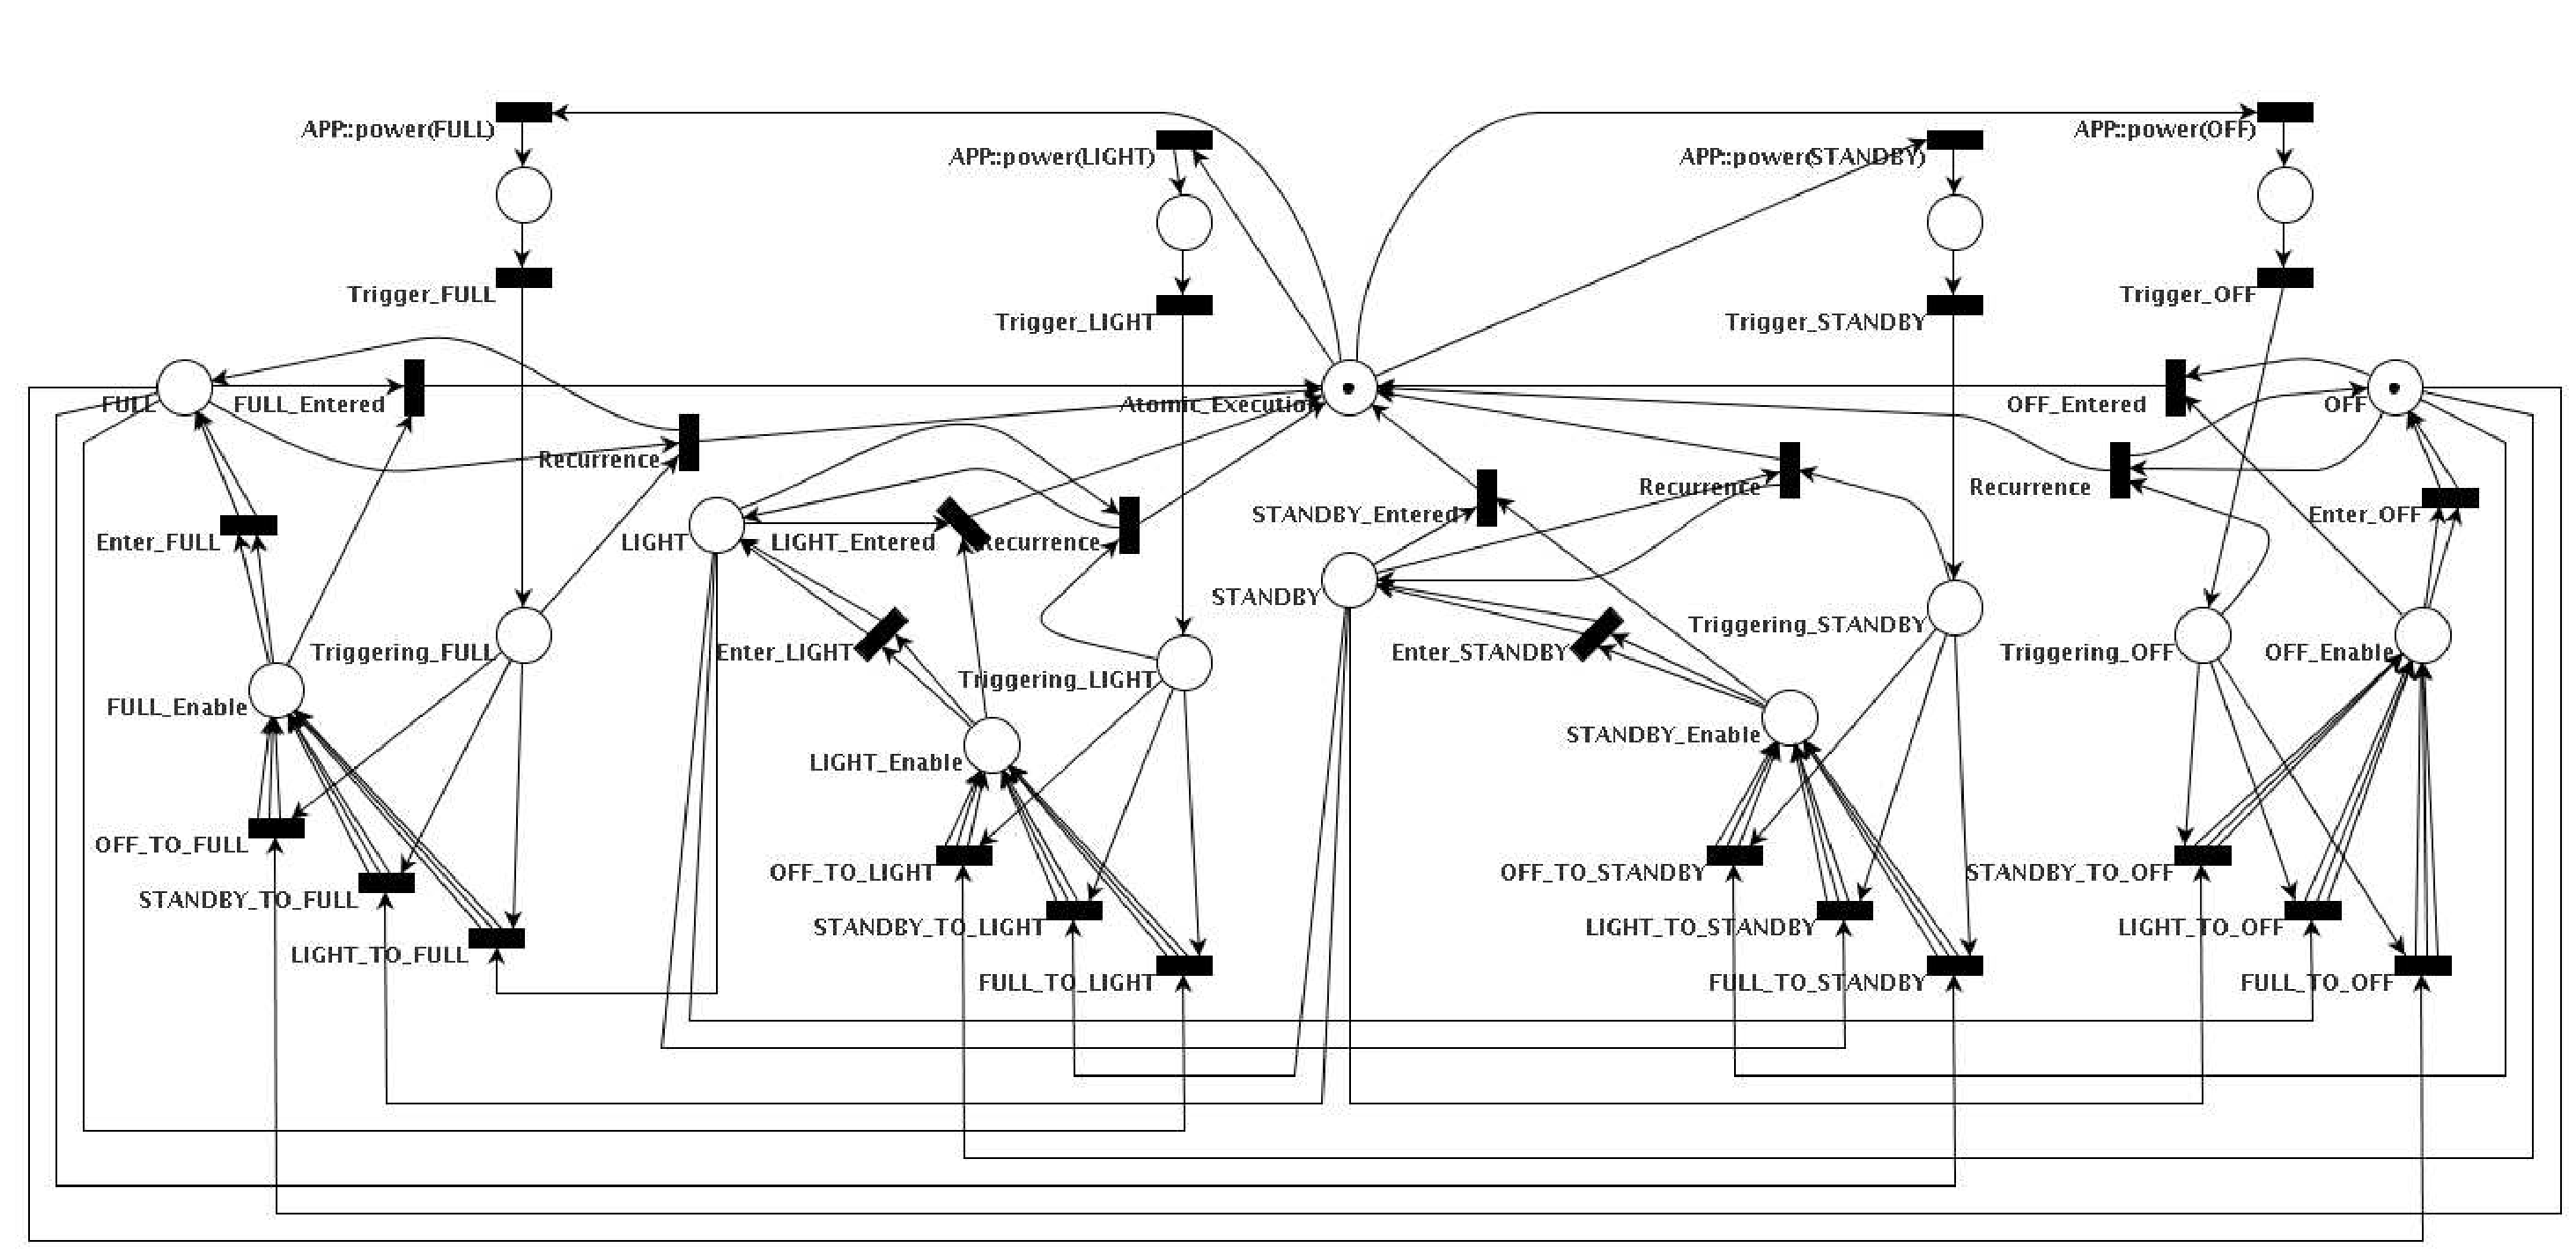
\includegraphics{fig/general_net}}}}\par}
%\end{figure}

\acks

Authors would like to thank Augusto Born de Oliveira, Hugo Marcondes,
Rafael Cancian and, specially, Prof. Jlio Zseremetta from Federal
University of Santa Catarina for very helpful discussion.

\bibliographystyle{plain}
\bibliography{power}

\end{document}
